\subsection{Halbleiter}

Unter einem Halbleiter wird in der Festkörperphysik ein Material bezeichnet, dessen Eigenschaften zwischen denen eines Leiters oder eines Isolators liegen.
Das elektrische Verhalten eines Stoffes wird durch den Energieabstand zwischen dem Leitungs- und dem Valenzband definiert.
Bei einem Leiter überlappen sich diese, wohingegen sie bei einem Isolator mindestens $\SI{4}{\electronvolt}$ weit auseinander liegen.
Bei einem Leiter befinden sich also genügend Ladungsträger im Leitungsband, wohingegen die aufzuwendende Energie für Isolatoren zu groß ist um das Valenzband zu verlassen.
Halbleiter weisen eine Bandlücke auf, die zwischen der eines Leiters und eines Isolators liegt.
Dies ist in Abbildung \ref{fig:bandschema} schematisch dargestellt.

\begin{figure}
  \centering
  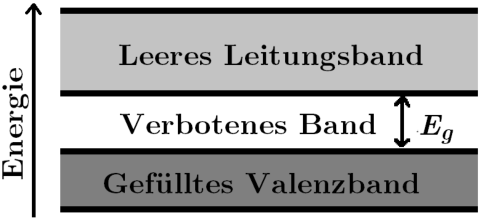
\includegraphics[width=0.5\textwidth]{content/graphics/Bandluecke.png}
  \caption{Bandschema eines gewöhnlichen Halbleiters wie Silizium.}
  \label{fig:bandschema}
\end{figure}

Silizium verfügt über vier Valenzelektronen, die für die Bindung mit den anderen Atomen genutzt werden.
Silizium weist eine Diamantstruktur mit vier nächsten Nachbarn auf, die alle über die entsprechenden Valenzelektronen verbunden werden.
Die grundlegende Leitfähigkeit eines Halbleiters ist von der Temperatur über thermische Anregungen abhängig.
Bei einer Temperatur von $\SI{0}{\kelvin}$ liegt keine elektrische Leitfähigkeit vor.
Durch die erwähnten thermischen Anregungen können die Elektronen ins Leitungsband angehoben werden.
Dadurch entsteht ein positiv geladenes "Loch", welches als ein Quasiteilchen mit effektiver Masse betrachtet werden kann.
Dabei ist die physikalische Beschreibung der Löcher analog zu den Elektronen, nur mit positiver Ladung.
Ohne ein äußeres elektrisches Feld rekombinieren das Elektron und das Loch erneut, da das Elektron immer noch über das Coulombfeld des Atomes gebunden ist.
Ein äußeres elektrisches Feld führt dann dazu, dass die Elektronen zur Anode und die Löcher in die andere Richtung wandern.
Dies wird Eigenleitung genannt.

Diese Leitfähigkeit lässt sich durch die sogenannte Dotierung, dem Einbringen von Fremdatomen, erhöhen.
Das Einbringen dieser Störstellen verringert die Bandlücke und erhöht die Leitfähigkeit.
Dabei werden abhängig von den eingebrachten Fremdatomen zwei Arten von Dotierungen in Halbleitern unterschieden.
Bei den n-typ Halbleitern wurden Atome eingebracht, die ein Elektron mehr im Valenzband aufweisen, wie z.B. Arsen.
Das überschüssige Elektron kann sich dann frei im Gitter bewegen.
Bei den p-typ Halbleitern wurden Atome eingebracht, die ein Elektron weniger im Valenzband aufweisen, wie z.B. Bor.
Somit fehlt innerhalb einer Bindung ein bindendes Elektron.
Durch Elektroneneinfang kann diese Lücke aufgefüllt werden.
Das Loch kann also als freier Ladungsträger mit positiver Ladung betrachtet werden.
Wird nun eine p- und n-dotierte Halbleiterschicht zusammen gebracht, so kommt es zum pn-Übergang.
Dies wird auch bei dem vorliegenden Siliziumstreifendetektor gemacht.
Aufgrund der Dotierung kommt es zu einer Ladungsträgerdiffusion zwischen den Schichten.
Die überschüssigen Ladungsträger der beiden Seiten rekombinieren miteinander.
Dadurch wird die p-Seite leicht positiv und die n-Seite leicht negativ geladen.
Es liegt somit ein Potentialunterschied vor, welcher Diffusionsspannung $U_D$ genannt wird.
Durch das Anlegen einer Spannung kommt es zu einer Ladungsträgerverarmung am pn-Übergang, da alle freien Ladungsträger durch das äußere Feld entzogen werden.
Dieser Bereich wird Sperrschicht genannt.
Die Dicke dieser Sperrschicht ist dabei abhängig von der angelegten Vorspannung und erreicht bei der Depletionsspannung $U_{dep}$ ihr Maximum, da sich die Depletionszone dann über den gesamten Kristall ausgebreitet hat.
Liegt also die Vorspannung unter der Depletionsspannung so ist nur ein kleiner Teil des Materials deplettiert.

Um nun die vollständige Energiedeposition eines ionisierenden Teilchens zu erfassen, muss der Sensor voll deplettiert sein.
Ansonsten würden die erzeugten Elektron-Loch-Paare umgehend mit den freien Ladungsträgern rekombinieren.
Innerhalb der Depletionszone kann es allerdings auch zu Leckstrom kommen.
Dieser entsteht durch die thermische Anregung die zur Entstehung von Elektron-Loch-Paaren führt und die Ladungsträger durch die angelegte Spannung zu den Polen geleitet werden.
Der Leckstrom steigt proportional zur Vorspannung an.
Dies ist in Abbildung \ref{fig:leckstrom} exemplarisch für das verwendete System dargestellt.
Dort ist zu erkennen, dass bis zu einer gewissen Spannung der Leckstrom stärker ansteigt.
An dieser Spannung ist der Kristall voll deplettiert, so dass der Leckstrom danach nur noch linear ansteigt.

\begin{figure}
  \centering
  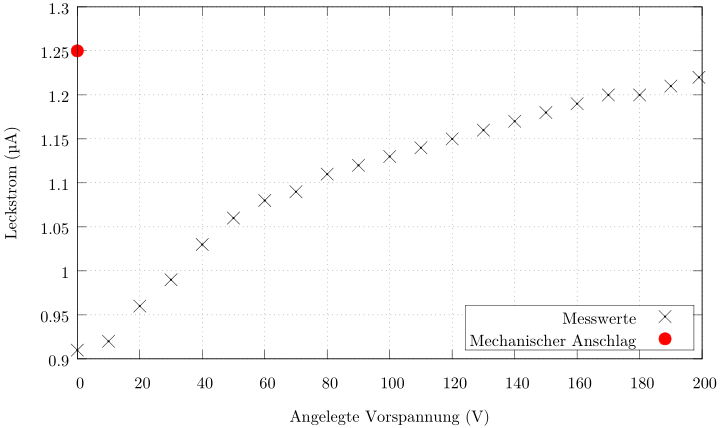
\includegraphics[width=0.8\textwidth]{content/graphics/leckstrom.png}
  \caption{Exemplarische Darstellung des Leckstroms anhand der Strom-Spannungs-Kennlinie des verwendeten Alibava Systems. Zu erkennen ist, dass bis zu einer gewissen Spannung der Leckstrom stärker ansteigt. Dort ist der Kristall voll deplettiert, so dass der Leckstrom danach nur noch linear ansteigt. Eingezeichnet ist außerdem der mechanische Anschlag. Durch Überdrehen des Spannungsreglers wird die Spannung minimal auf Durchlassrichtung angelegt und der Sensor an sich wird leitend.}
  \label{fig:leckstrom}
\end{figure}

















%
